\section{Box-Jenkins analysis} 

Before going further and select a model that will be able to predict the air temperature in Recife for the months following the year $1995$, we need to detrend and deseasonalize our time serie. 

% TODO: explain why we need stationary time series

\subsection{Differencing}

We first remove the seasonality by taking a seasonal difference which consist by taking the difference between an observation and the previous observation at the same season (in our case, $12$ months before): $X'_t = X_t - X_{t-12}$. 
Then, we remove the trend by first differencing the serie.

\begin{figure}[H]
	\centering
	\begin{subfigure}{0.49\textwidth}
		\centering
		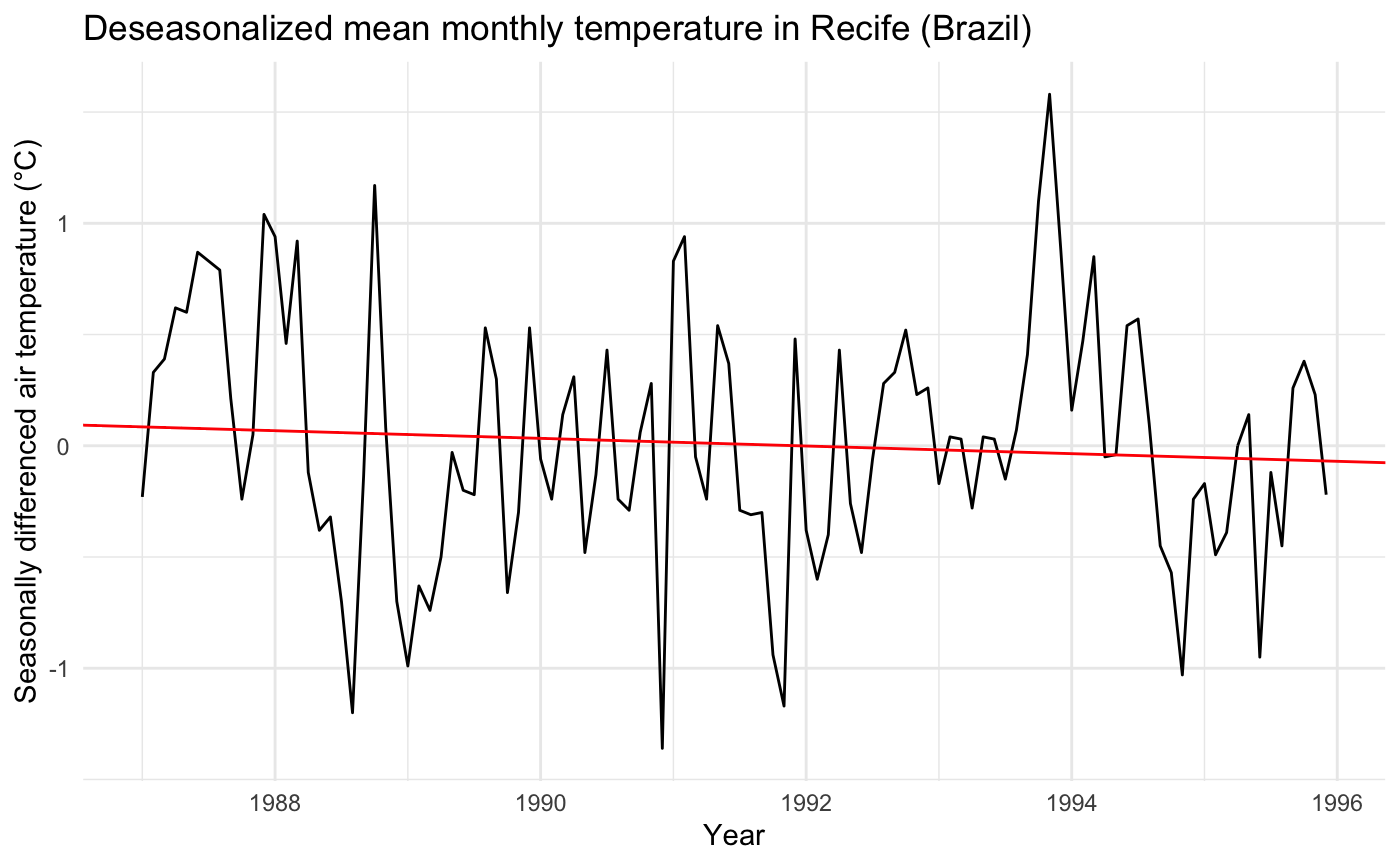
\includegraphics[width=\textwidth]{figures/box_jenkins/deseasonalized_time_serie.png}
		\label{fig:deseasonalized-time-serie}
	\end{subfigure}
	\begin{subfigure}{0.49\textwidth}
		\centering
		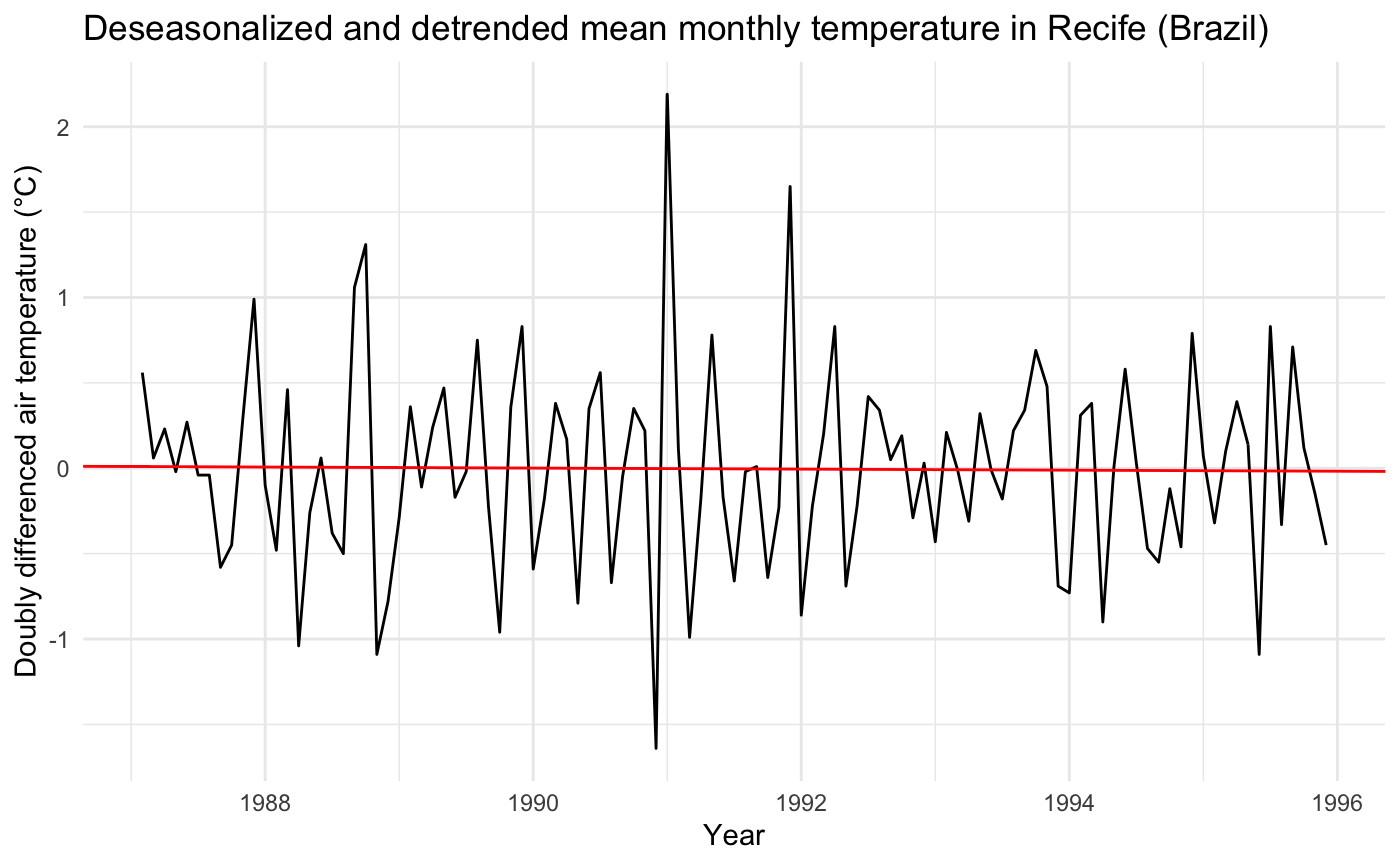
\includegraphics[width=\textwidth]{figures/box_jenkins/doubly_differenced_time_serie.png}
		\label{fig:doubly-differenced-time-serie}
	\end{subfigure}
	\caption{Deseasonalized time serie (at left) and doubly differenced time serie (deseasoned and detrended) (at right). In red is the regression line.}
\end{figure}

After doubly differencing, the time serie is now stationary as shown on the plots above.

\subsection{Model intuition with ACF and PACF plots}

We can now go further and analyse the autocorrelation and partial autocorrelation plots (ACF, PACF) of our stationary time series to have an intuition about the possible model we could choose to modelize our serie.

% TODO: explain briefly SARIMA for seasonal time series
Because we are dealing we seasonal data, we will probably use a SARIMA model which consists in adding additional seasonal terms to the ARIMA model, 
\begin{equation}
	\underbrace{(p, d, q)}_{\text{non-seasonal part}} \times \underbrace{(P, D, Q)_m}_{\text{seasonal part}}
\end{equation} 
where \textbf{p}, \textbf{d} and \textbf{q} (\textbf{P}, \textbf{D} and \textbf{Q}) are respectively the orders of the non-seasonal (seasonal) AR-process, difference and MA-process whereas \textbf{m} is the number of observations per year (in our case $m = 12$).

On a yearly basis, up to a lag of $8$ years, the ACF converge toward zero likewise the PACF. However, we notice a significant spike at lag $12$ for the ACF suggesting a seasonal MA($1$) component. In the same idea, the PACF shows a significant spike at lag $12$ as well suggesting a seasonal AR($1$) component.

\begin{figure}[H]
	\centering
	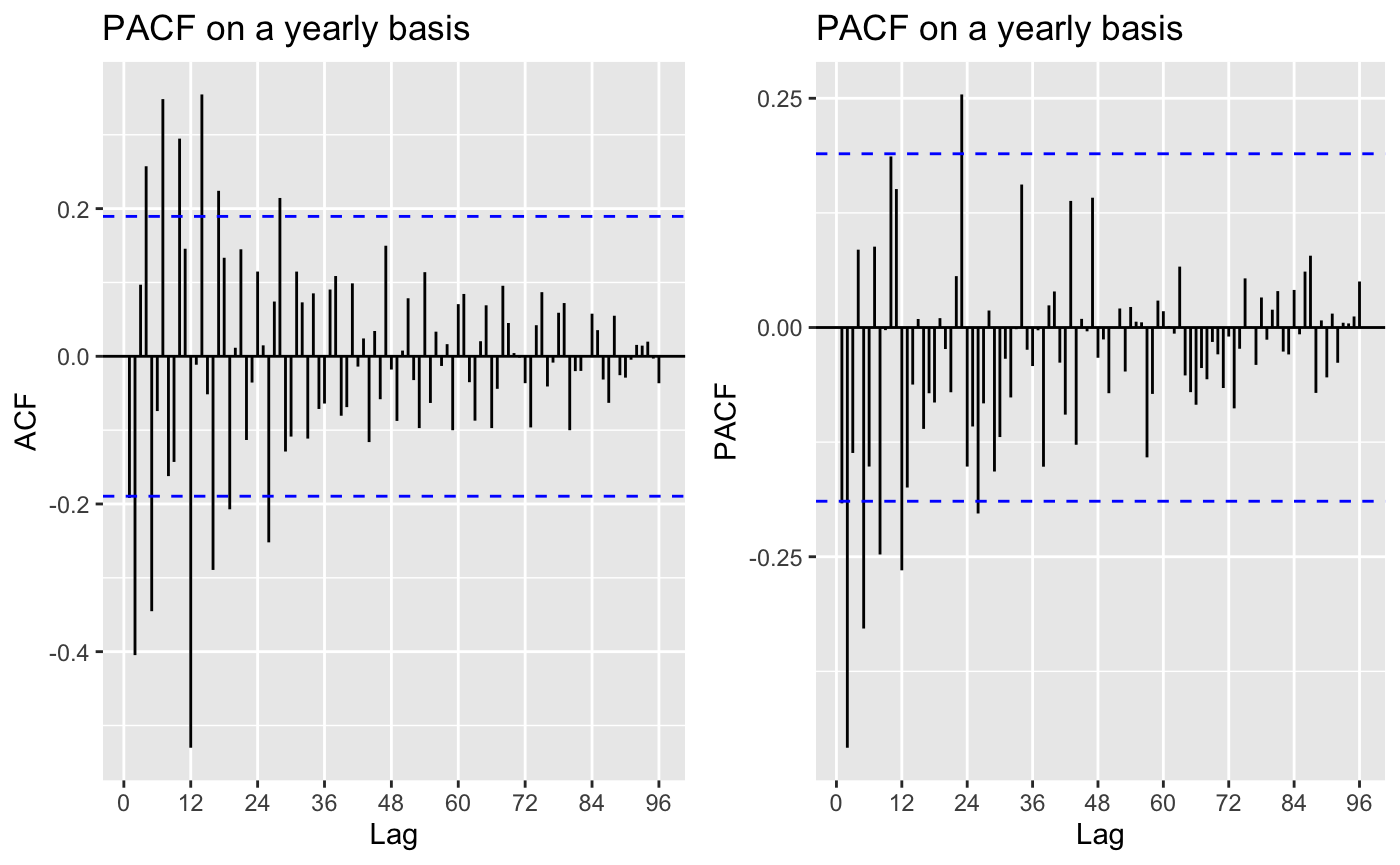
\includegraphics{figures/box_jenkins/yearly_acf_pacf.png}
	\caption{ACF and PACF plots on a yearly basis}
	\label{fig:yearly-acf-pacf}
\end{figure}

We can restreint ourselve to a monthly basis to check for any non-seasonal components. We have $5$ significant spikes respectively at lag $2$, $4$, $5$, $7$ and $10$ for the ACF suggesting a non-seasonal MA($5$) component. On the other hand, we have $3$ significant spikes at lag $2$, $5$ and $8$ for the PACF suggesting a non-seasonal AR($3$) component. 

\begin{figure}[H]
	\centering
	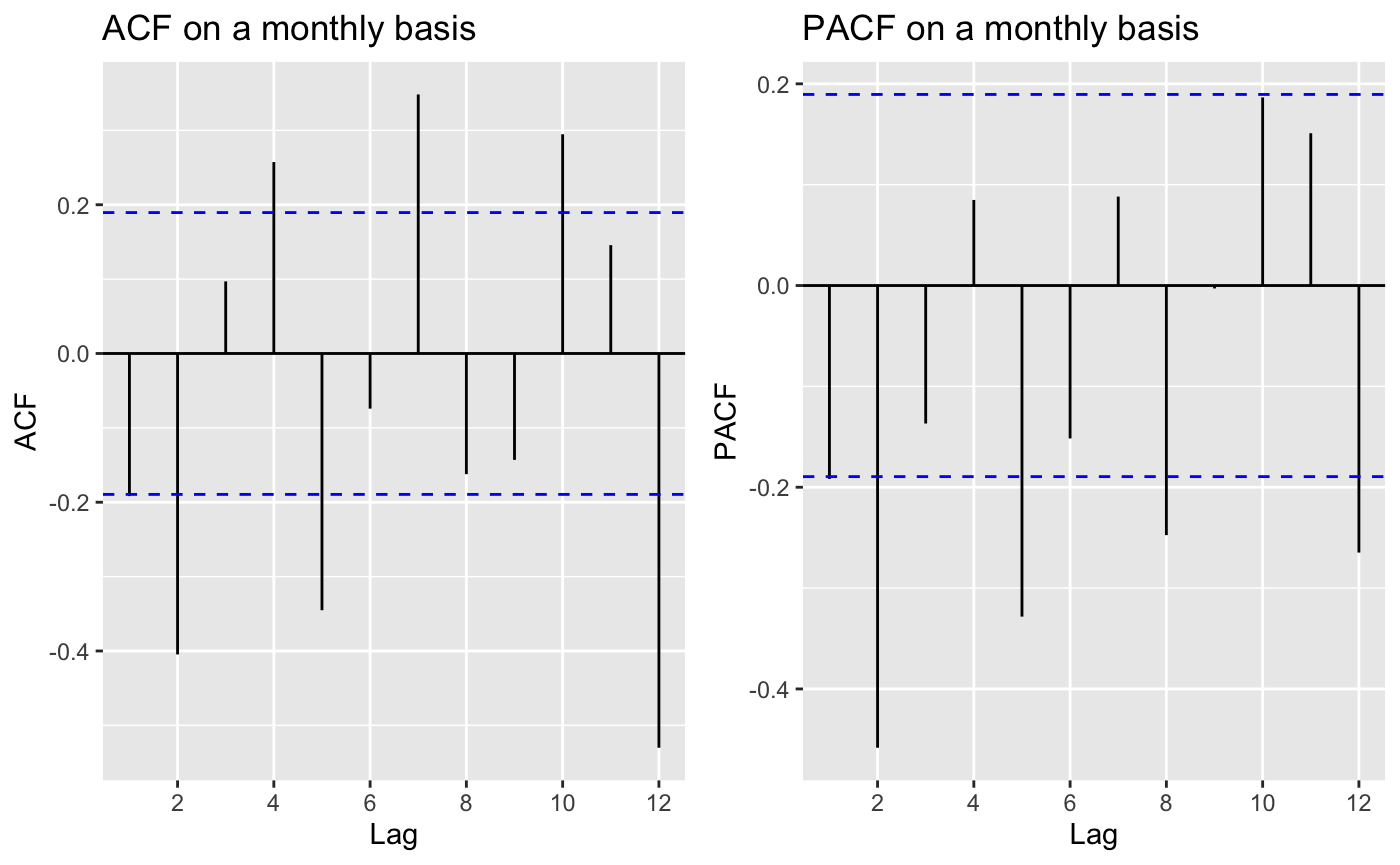
\includegraphics{figures/box_jenkins/monthly_acf_pacf.png}
	\caption{ACF and PACF plots on a monthly basis}
	\label{fig:monthly-acf-pacf}
\end{figure}

Finally, with all these considerations, our first intuition is to modelize our time serie with the following SARIMA process,

\begin{equation}
	(3, 1, 5) \times (1, 1, 1)_{12}
\end{equation}

But because of the decay in ACF and PACF on a yearly basis, we could as well modelize with these two other SARIMA processes,

\begin{equation}
	\begin{array}{rl}
		(3, 1, 5) \times (0, 1, 1)_{12} \quad ; \quad (3, 1, 5) \times (1, 1, 0)_{12}
	\end{array}
\end{equation}

\subsection{Automatic model selection with AIC and BIC}

After guessing the ideal model, we perform model selection for p and q up to $4$ and $6$ respectively because both ACF and PACF plots have at least one spike near outside the confidence interval. We also choose P and Q both up to $1$. Below are the top $10\%$ models based on the AIC criterion. We chose to also compute the BIC (as the AIC tend to overestimate the number of parameters) and the log likelihood.

\begin{figure}[H]
	\centering
	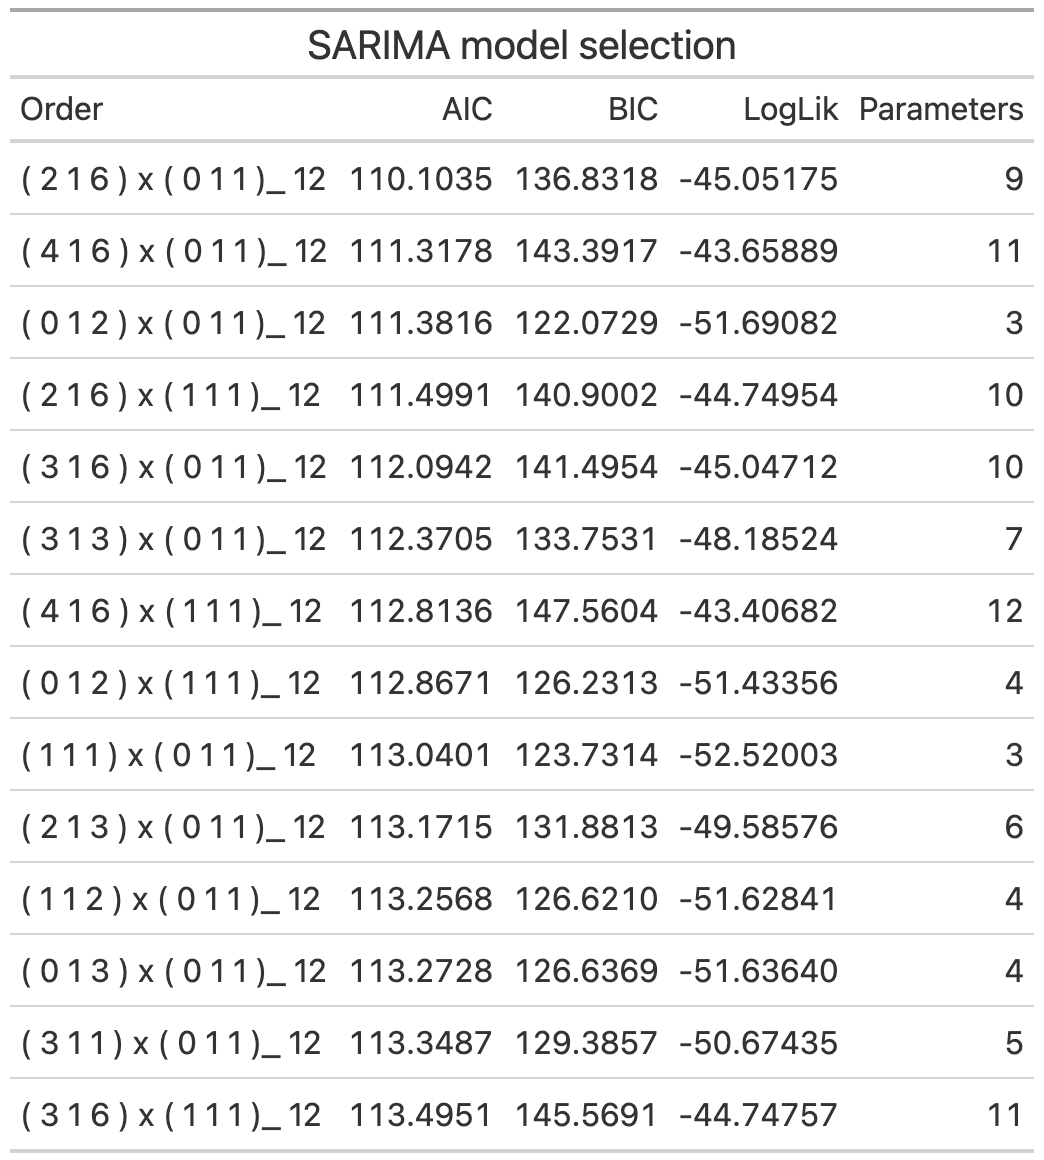
\includegraphics[width=0.5\textwidth]{figures/box_jenkins/sarima_model_selection.png}
	\caption{Summary of the 10\% best SARIMA models based on the AIC}
	\label{fig:sarima-model-selection}
\end{figure}

We notice that our intuition was not that bad but we will favour simpler models. Therefore, based on these results, we choose the third model on the list because it has way fewer parameters than the two firsts. The BIC for that model is also the lowest in that list. Thus, that is the following SARIMA-process,
\begin{equation}
	\text{model 1}: \quad (0, 1, 2) \times (0, 1, 1)_{12}
\end{equation}
that presents only $3$ parameters.

Nevertheless, we will compare it with a model that has one more parameter,
\begin{equation}
	\text{model 2}: \quad (0, 1, 2) \times (1, 1, 1)_{12}
\end{equation}

We could also compare it with, 
\begin{equation}
	\text{model 3}: \quad (1, 1, 1) \times (0, 1, 1)_{12}
\end{equation}

\subsection{Model validation}

\subsubsection{Coefficients significance}

We first want to verify that the coefficients of our model are statistically significants. To do that, we perform the following univariate two sided hypothesis test which is based on a normal approximation,

\begin{align*}
	H_0&: \text{coeff}(i) = 0 \\
	H_1&: \text{coeff}(i) \neq 0
\end{align*}
for $i = 0,\dots,(p + P) + (q + Q)$.

The results are the summarized in the following tables,
\begin{table}[H]
	\centering
	\begin{tabular}{|c|l|l|l|}
		\hline
		\textbf{model 1}    & ma1			& ma2			& ma3 \\\hline
		    /				& $3.02e-7$ 	& $2.136e-3$ 	& 6.35e-6 \\\hline
	\end{tabular}
	\caption{p-value for univariate two sided test for coefficients significant of model 1}
	\label{tab:coefficients-significance-model1}
\end{table}

\begin{table}[H]
	\centering
	\begin{tabular}{|c|l|l|l|l|}
		\hline
		\textbf{model 2}    & ma1			& ma2			& sar1		 & sma1		 \\\hline
		    /				& $2.639e-7$ 	& $3.558e-3$ 	& $4.674e-1$ & $1.95e-2$ \\\hline
	\end{tabular}
	\caption{p-value for univariate two sided test for coefficients significant of model 2}
	\label{tab:coefficients-significance-model2}
\end{table}

\begin{table}[H]
	\centering
	\begin{tabular}{|c|l|l|l|}
		\hline
		\textbf{model 3}    & ar1			& ma1			& sma1 \\\hline
		    /				& $7.982e-7$ 	& $8.393e-25$ 	& $2.277e-7$ \\\hline
	\end{tabular}
	\caption{p-value for univariate two sided test for coefficients significant of model 3}
	\label{tab:coefficients-significance-model3}
\end{table}

Based on this analysis, for a level of significance of $5\%$, we can reject our second model as it has one coefficient not statistically significant and we conclude that it is better to consider a model with $3$ coefficients.

\subsubsection{Residual analysis}

We want to check if there is any correlation in the residuals of our models. To do that, we perform a \textit{Ljung-Box test} on the residuals which consists in the following hypothesis,
\begin{align*}
	H_0&: \textit{the residuals are independently distributed.} \\
	H_1&: \textit{the residuals are not independently distributed. They exhibit serial correlation instead.}
\end{align*}

% TODO: plot of Ljung-Box test + Normality of residuals.

\begin{figure}[H]
	\centering
	\begin{subfigure}{0.49\textwidth}
		\centering
		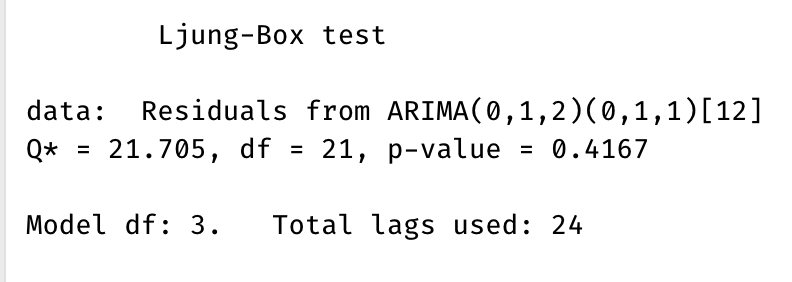
\includegraphics[width=\textwidth]{figures/box_jenkins/ljung_box_test_model1.png}
		\label{fig:ljung-box-test-model1}
	\end{subfigure}
	\begin{subfigure}{0.49\textwidth}
		\centering
		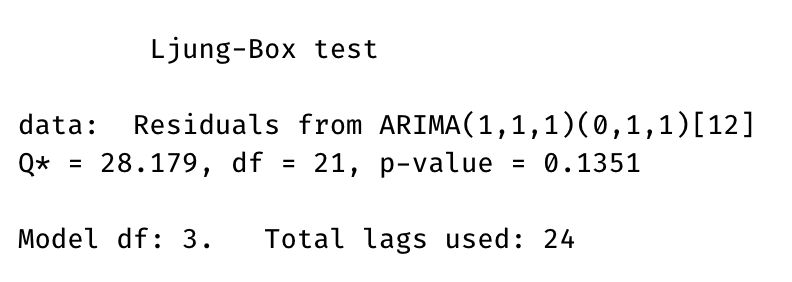
\includegraphics[width=\textwidth]{figures/box_jenkins//ljung_box_test_model3.png}
		\label{fig:ljung-box-test-model3}
	\end{subfigure}
	\caption{Ljung-Box test for model 1 (at left) and model 3 (deseasoned and detrended) (at right).}
\end{figure}

All the three models pass the Ljung-Box test at $5\%$ significance level. Then, the residuals are not correlated and we should have an accurate prediction interval. Moreover, the residuals are more or less normals (\autoref{fig:residuals_analysis_model1}, \autoref{fig:residuals_analysis_model2})

\subsubsection{Predictive power}

Despite our models passing the Ljung-Box test, we want to ensure they have good predictive power by comparing the last $20\%$ (i.e. last two years) of the original time serie with a forecast for these same $20\%$ using our models.

\begin{figure}[H]
	\centering
	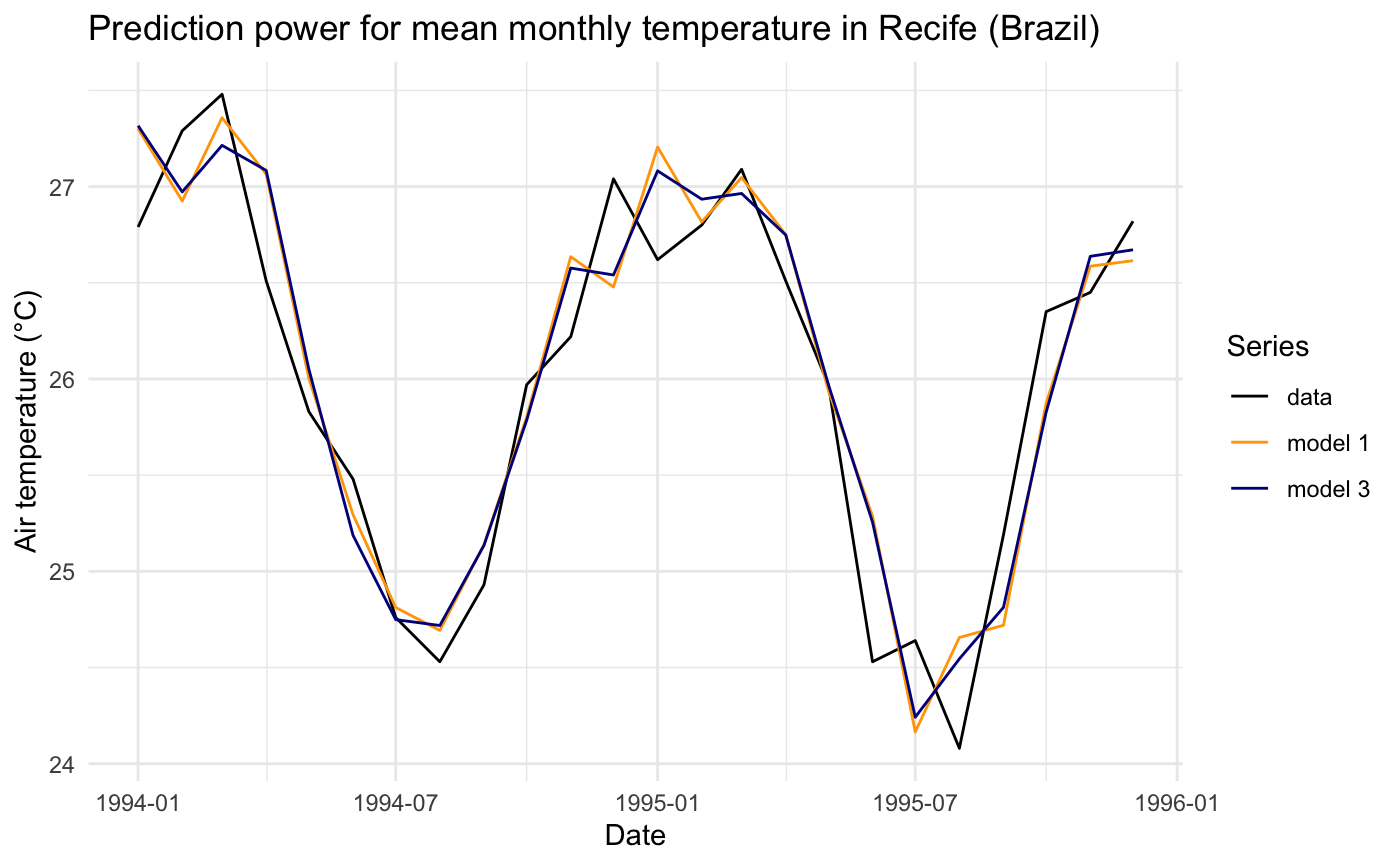
\includegraphics{figures/box_jenkins/predictive_power.png}
	\caption{Predictive power of the two SARIMA models (1 and 3) compared with the last two years of the original data (\textit{in dotted black}).}
	\label{fig:predictive-power}
\end{figure}

...

Looking at the MSE of the prediction, we notice that the model 3 is slightly better than model 1 with an MSE of $0.134$.
\begin{figure}[H]
	\centering
	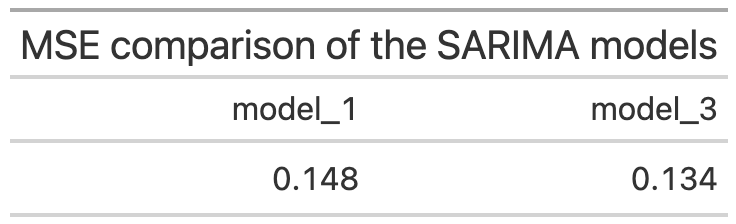
\includegraphics[width=0.5\textwidth]{figures/box_jenkins/predictive_power_mse.png}
	\caption{Predictive power of the two SARIMA models (1 and 3).}
	\label{fig:predictive-power-mse}
\end{figure}

Therefore, we choose to keep the model $3$ as the final model for forecasting. This model $(1, 1, 1) \times (0, 1, 1)_{12}$ can be written the following way,

\begin{equation} \label{eq:final-model}
	(1 - \phi_1 B)(1 - B)(1 - B^{12}) = (1 + \theta_1 B)(1 + \Theta_1 B^{12}) \varepsilon_t
\end{equation}
where $B$ is the \textit{"backshift operator"} and $\phi_1 = 0.3529$, $\theta_1 = -0.8946$, $\Theta_1 = -0.9999$.